% !TEX root= ../main.tex
\section{Results in Kernel Theory}
\label{sec:Results in Kernel Theory}
The end goal within Kernel Theory is ultimately to develop an easy way of answering the question ``Does this digraph have a kernel?'' no matter the graph, and no matter the answer.
As of today, we are not quite there, but a lot of work has been put into trying to identify special circumstances under which one is guaranteed to have (or guaranteed to not have) a kernel in the given graph.
One significant result is the theorem proven by Moses Richardson in 1953:
\begin{theorem}[\cite{am-richardson}]
  If D is a finitary digraph without odd cycles, then D has a kernel.
\end{theorem}
Intuitively, one might be tempted to believe that \textit{all} digraphs without odd cycles have kernels, but this is not the case.
Until now, all our paradoxes have been statements that -- directly or indirectly -- have been referring back to themselves (giving cycles in the graph) and thus causing a logical conflict, and it is hard to imagine any other way to construct paradoxical statements.
The following construction will however reveal our lack of imagination.

The \textit{Yablo Graph}\cite{analysis-yablo} is an example of an acyclic graph with no kernel.
It is constructed with an infinite set of vertices $\{ x_i \;|\; i \in \mathbb{N} \}$ and a set of edges $N$ such that $\langle x_i, x_j \rangle \in N$ iff $i < j$.\par
\begin{figure}[!h]
  \centering
  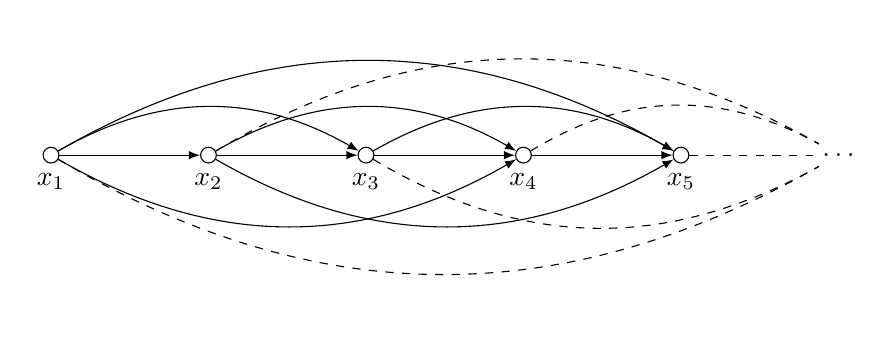
\begin{tikzpicture}
    [
    point/.style={circle,draw,inner sep=0pt,minimum size=2mm},
    collection/.style={thick,rectangle,draw,inner sep=0pt,minimum height=14mm, minimum width= 9mm}
    ]
    \node (1) at (0,1) [point,label=below:$x_1$] {};
    \node (2) at (2,1) [point,label=below:$x_2$] {};
    \node (3) at (4,1) [point,label=below:$x_3$] {};
    \node (4) at (6,1) [point,label=below:$x_4$] {};
    \node (5) at (8,1) [point,label=below:$x_5$] {};
    \node (6) at (10,1) [] {$\dots$};
    \draw [-latex] (1) to (2);
    \draw [-latex] (2) to (3);
    \draw [-latex] (3) to (4);
    \draw [-latex] (4) to (5);
    \draw [dashed] (5) to (6);
    \draw [-latex, bend left] (1) to (3);
    \draw [-latex, bend left] (2) to (4);
    \draw [-latex, bend left] (3) to (5);
    \draw [dashed, bend left] (4) to (6);
    \draw [-latex, bend right] (1) to (4);
    \draw [-latex, bend right] (2) to (5);
    \draw [dashed, bend right] (3) to (6);
    \draw [-latex, bend left] (1) to (5);
    \draw [dashed, bend left] (2) to (6);
    \draw [dashed, bend right] (1) to (6);
  \end{tikzpicture}
  \caption{The Yablo Graph}
  \label{fig:yablo-graph}
\end{figure}
Since there exist no two numbers $x,y \in \mathbb{N}$ such that $x < y$ and $y < x$, we get that the Yablo-graph indeed is acyclic.
Furthermore, since any natural number has infinitely many numbers strictly larger than it, we get that all the vertices are infinitely branching, making the Yablo-graph infinitary.

The discourse represented by the Yablo-graph would -- informally -- be the situation with an infinite number of statements, all saying ``Every statement after this statement is false''.

We will later show formally that the Yablo-graph is indeed without a kernel, but for now the following explanation should suffice.

Suppose that the Yablo-graph \textit{has} a kernel and that the vertex $x_a$ is in it.
Then all the vertices to the right of $x_a$ are necessarily outside of the kernel, including $x_{a+1}$.
But if $x_{a+1}$ is outside of the kernel, it has to point to a vertex on the inside.
This is now impossible, since the out-neighborhood of $x_{a+1}$ is a subset of the out-neighborhood of $x_a$.
Since $x_a$ was chosen without any restrictions, no vertex can be inside the kernel, making it empty.
Since no kernel can be empty, we have a contradiction, making the Yablo-graph without a kernel.

One thing should be mentioned at this point:
The inverse of Richardson's statement is not valid; neither odd cycles nor infinitely branching vertices \textit{entail} that their respective graphs are paradoxical.
The following two graphs illustrate this point:\par
\begin{figure}[!h]
  \centering
  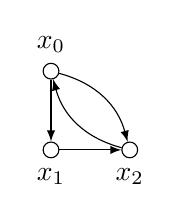
\begin{tikzpicture}
    [
    point/.style={circle,draw,inner sep=0pt,minimum size=2mm},
    collection/.style={thick,rectangle,draw,inner sep=0pt,minimum height=14mm, minimum width= 9mm}
    ]
    \node (0) at (0,1) [point,label=above:$x_0$] {};
    \node (1) at (0,0) [point,label=below:$x_1$] {};
    \node (2) at (1,0) [point,label=below:$x_2$] {};
    \draw [-latex] (0) to (1);
    \draw [-latex] (1) to (2);
    \draw [-latex, bend left] (2) to (0);
    \draw [-latex, bend left] (0) to (2);
  \end{tikzpicture}
  \caption{}
  \label{odd_cycle_with_kernel}
\end{figure}
The above graph contains an odd cycle, but the singleton set $\{x_2\}$ is a kernel.\par
\begin{figure}[!h]
  \centering
  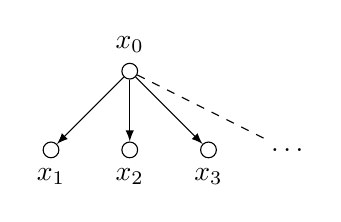
\begin{tikzpicture}
    [
    point/.style={circle,draw,inner sep=0pt,minimum size=2mm},
    collection/.style={thick,rectangle,draw,inner sep=0pt,minimum height=14mm, minimum width= 9mm}
    ]
    \node (0) at (1,2) [point,label=above:$x_0$] {};
    \node (1) at (0,1) [point,label=below:$x_1$] {};
    \node (2) at (1,1) [point,label=below:$x_2$] {};
    \node (3) at (2,1) [point,label=below:$x_3$] {};
    \node (4) at (3,1) [] {$\dots$};
    \draw [-latex] (0) to (1);
    \draw [-latex] (0) to (2);
    \draw [-latex] (0) to (3);
    \draw [dashed] (0) to (4);
  \end{tikzpicture}
  \caption{}
  \label{infinitary_with_kernel}
\end{figure}
The above graph has an infinitely branching vertex $x_0$, but the infinite set $\{x_i \;|\; x > 0\}$ is a kernel.

Another important theorem within kernel theory is shown by Roy T. Cook in \cite{cook}, stating that every digraph with at least one edge can be transformed into an infinitary dag -- preserving and reflecting the solutions.
This means that for any finitary graph that is paradoxical by the virtue of having an odd cycle, there is a corresponding infinitary, \textit{acyclic} digraph that is also paradoxical.
So if one is trying to find ways to identify paradoxical graphs, one does only need to look at dags.
